\section{Исследование и построение решения задачи}
\label{sec:Chapter3} \index{Chapter3}

Для того, чтобы внедрить наше решение в существующий проект по разработке компилятора MyTS,
сначала необходимо тщательно изучить его внутреннее устройство.
Составим обзор компонент компилятора для понимания, как сделать наше решение качественной и логичной частью всего проекта.

\subsection{Исследование компонент компилятора}

\subsubsection{Лексический анализ}

Этот компонент преобразует исходный код в последовательность токенов.
Входные данные должны быть корректной строкой UTF8.
Токены могут быть литералами, знаками препинания или ключевыми словами, представленными свойством \hl{Token::type}.
Поскольку JS содержит контекстуальные ключевые слова, например, \hl{static} - это ключевое слово внутри тела класса,
но в других местах это простой идентификатор, токены имеют дополнительное поле \hl{Token::keywordType},
которое всегда соответствует соответствующему ключевому слову независимо от реального \hl{Token::type}.
Поскольку на этом уровне могут возникать синтаксические ошибки, лексер может выдавать соответствующую ошибку.

\subsubsection{Область видимости}

Структуры \hl{binder::Scope} - это конструкции, в которых хранятся переменные.
Каждая область видимости имеет родителя - область по вложенности выше, все объявления \hl{binder::Decl},
которые хранятся в таблице переменных \hl{Scope::bindings}.
Эта таблица содержит строку в качестве ключа и переменную \hl{binder::Variable} в качестве значения.

\subsubsection{Объявления}

Объявления типа \hl{var a} или \hl{let b} во время синтаксического анализа преобразуются в \hl{binder::Decl}.
Каждое объявление знает имя и AST-узел, с которым оно связано.

\subsubsection{Переменные}

Переменные по умолчанию не создаются.
Декларации преобразуются в переменные, если они проходят проверку в рамках области видимости.
Структура переменной \hl{binder::Variable} содержит в себе объявление, из которого она взята, а также имеет
\hl{checker::Type}, который будет представлять фактический статический тип переменной.
Этот тип неизвестен во время синтаксического анализа и заполняется позже компонентом \hl{Checker}.

\subsubsection{Binder}

Этот компонент создает и проверяет все привязки(bindings) деклараций к области видимости.
Сам по себе он не является отдельным анализом.
Каждая проверка привязки запускается в процессе синтаксического анализа.
В настоящее время триггерами могут быть:

\begin{itemize}[left=2em]
    \item Создание новой области видимости.
    \item Добавление объявления в текущую область видимости.
    Если она не может добавить привязку, возникает синтаксическая ошибка.
\end{itemize}

\subsubsection{Парсер}

Парсер является одним из основных компонент и взаимодействует с binder-ом и лексером одновременно.
Синтаксический анализ является однопоточным, и входные данные обрабатываются только один раз.
Для парсинга выбран синтаксический анализатор LR(1), поэтому он видит только следующий токен,
но может заглянуть в следующую точку кода.
Однако из-за новых возможностей стандарта ES2015 список параметров лямбда функций и шаблоны деструктурирования
больше не могут быть корректно прочитаны, заглядывая только на один токен вперед.
В этих сценариях синтаксический анализатор работает в отказоустойчивом режиме, что означает,
что он следует менее строгой грамматике, чем стандартная.
Всякий раз, когда закрывающий токен для этих языковых элементов найден или не найден, выполняется обход построенного AST
дерева и проверка его правильности в соответствии с правилами грамматики.
По мере того как AST строится во время синтаксического анализа, также создается дерево областей видимости.
Как только парсер обрабатывает очередной блок кода или функцию, запускается binder, который создает для них новую область
видимости и привязывает их к ней.
Поскольку время жизни этих областей совпадает со временем жизни соответствующих узлов AST дерева,
структуры представляющие узел также сохраняют у себя эти области видимости.
Всякий раз, когда считано объявление переменной, запускается binder для проверки привязки.
Таким образом, в общем случае синтаксический анализатор уведомляет binder только о том, что он обнаружил
новое начало области видимости или объявление новой переменной.

\subsubsection{AST дерево}

ASTNode - это базовый класс всех узлов, сгенерированных парсером.
Узел AST хранит в себе данные о позиции в исходном коде, родительский узел и другие атрибуты,
которые добавляются дочерним классам при наследовании.

\subsubsection{Анализ имен переменных}

После того, как исходный код обработан парсером, AST проходит анализ имен переменных.
После него создается класс программы, содержащий AST дерево, позиции переменных в исходном коде и некоторые метаданные.
Главной целью этого анализа является определение типа переменной для обеспечения эффективной многопоточной компиляции
без блокировки, не считая планирования потоков.
Переменная может быть локальная или лексическая.
Во время обхода AST дерева мы ссылаемся на уже сгенерированные области видимости, присвоенные statement узлам,
чтобы определить, в какой области мы на самом деле находимся.
Всякий раз, когда мы оказываемся в узле идентификатора переменной \hl{ir::Identifier},
анализатор пытается разрешить ее тип из текущей области.
Если у переменной нет конфликтов с какой-либо другой переменной из области видимости \hl{binder::VariableScope}
(чаще всего это \hl{binder::FunctionScope}, иногда \hl{binder::LoopScope}), переменная объявляется как локальная.
В противном случае она получает лексический индекс из ближайшей области видимости и помечается как лексическая.
Каждый раз, когда из области видимости запрашивается лексический слот на переменную, область становится лексической.
Это означает, что во время компиляции в начале функции должно быть создано так называемое лексическое окружение.
В этом анализе мы также определяем, является ли локальная переменная внутри объявления цикла частью замыкания
внутри его тела.
Результат этого анализа определяет, должны ли цикл или его декларация быть лексическими или нет.
Таким образом, перед переходом непосредственно на стадию кодогенерации AST обрабатывается только один раз.
Каждая область видимости содержит в себе информацию о том, нуждается ли она в лексическом окружении или нет,
и каждая переменная знает, является ли она лексической или нет.

\subsubsection{Чекер}

Этот компонент семантически анализирует код, используя AST дерево, области видимости и переменные.
Чекер обходит AST дерево и проверяет каждый узел, используя виртуальную функцию \hl{Checker},
перегруженную для всех узлов по-своему.
Когда чекер обнаруживает узел с объявлением какой-то переменной, он выполняет ее поиск во всех областях видимости
по степени их вложенности друг в друга.
Как только найдено объявление этой переменной в какой-то области видимости, чекер присваивает тип выражения к узлу
дерева, если он задан явно, либо использует для этого вывод типов.

\begin{itemize}[left=2em]
    \item При незаданной аннотации, тип объявленной переменной выводится с помощью инициализатора.
    \item При объявлении функции чекер создает для нее сигнатуру, которая состоит из параметров в заданном порядке
    и типа возвращаемого значения.
    Оно в свою очередь выводится из явно указанной аннотации типа или выражения, следующего за return в теле функции.
    \item При объявлении интерфейса чекер создает объектный тип, который хранит в себе все поля и их типы, а также
    сигнатуры методов и конструкторов интерфейса.
    \item При объявлении псевдонима типа чекер использует тип, который этому псевдониму и присваивается.
\end{itemize}

\subsubsection{TsType}

Как только тип объявления вычислен, ему присваивается значение ts-типа объявленной переменной.
Используя структуру \hl{checker::Type}, чекер может проверять на валидность выражения присваивания, бинарные или унарные
операции, вызовы функций и конструкторов, доступы к полям класса и наследование.
Важно отметить, что statement не создает тип, это делают только выражения.

\begin{itemize}[left=2em]
    \item Statement проверяется только семантически.
    Например, если statement проверяется на наличие у него выражения-условия,
    которое вычисляется в тип void, то чекер сообщает об ошибке, поскольку выражения типа void не могут быть
    проверены на истинность.
    \item Выражения, с другой стороны, по своей сути порождают типы.
    Например, бинарное выражение \hl{5 + 6} порождает числовой тип.
    Вот почему функция \hl{ASTNode::Check} узла statement всегда возвращает значение nullptr, а функция \hl{ASTNode::Check} узла
    выражения всегда возвращает тип, созданный этим выражением.
\end{itemize}

\subsubsection{Отношения}

В определенный момент во время семантического анализа чекер должен соотнести различные типы друг с другом.
Например, если переменной присвоено значение a = 15, чекер сравнивает тип переменной a с типом
инициализатора, который представляет собой числовое литеральное выражение, приводимое к числовому типу.
Если a был объявлен как \hl{let a: string}, то это присвоение приведет к ошибке, поскольку тип string не может быть
присвоен типу number.
В зависимости от операции, используемой с переменными, существует 3 различных отношения типов:

\begin{itemize}[left=2em]
    \item Отношение идентичности: отношение является истинным, если два сравниваемых типа абсолютно идентичны.
    Оно используется при повторном объявлении переменной или поля, и это наиболее сильное отношение.
    \item Отношение присваивания: отношение является истинным, если тип с правой стороны может быть присваивоен типу
    с левой стороны.
    Оно используется при обработке присваиваний, операндов бинарных выражений, наследования (отношение базового и дочернего класса),
    а также для проверки совместимости типа возвращаемых выражений из return с типом возвращаемого значения, объявленного в функциях.
    \item Отношение приводимости: отношение является истинным, если тип в правой части может быть приведен к типу в левой части.
    Оно используется при работе с операторами сравнения, приведения типов и в не сильно отличается от отношения присваивания.
    Это самое слабое отношение.
\end{itemize}

\subsubsection{Сигнатуры функций}

Сигнатуры создаются для функций и методов, и они могут быть явно объявлены в теле интерфейса или класса,
используя следующий синтаксис: \hl{(a: number, b: string): number}.
Существует два типа сигнатур: сигнатуры функций и конструкторов.
Сигнатуры функций используются для проверки правильности вызовов функций.
Например, если объявление функции с именем func1 было объявлено с сигнатурой (a: string, b: string), то оно не может
быть вызвано с меньшим или большим количеством параметров, чем 2, и аргументы вызова функции должны быть присваиваемы
типу параметра сигнатуры в правильном порядке.
Таким образом, чекер выдаст ошибку в любом из этих случаев:
func1(1), func1(1, 2, 3), func1("foo"), func1(2, "bar").
Сигнатуры конструкторов идентичны по своим правилам.
Разница лишь в том, что они используются при создании объектов и, соответсвенно, в выражения с ключевым словом new.

\subsubsection{Lowering фазы}

Lowering преобразование - это фаза трансформаций, работающая после чекера и перед кодогенерацией,
во время которой происходит обход AST дерева, преобразуя некоторые его узлы и заменяя отфильтрованные выражения более
простыми и низкоуровневыми конструкциями.
Стоит уточнить, что не все фазы lowering-а проходят после чекера.
На самом деле, некоторые проходы трансформируют AST дерево и до семантического анализа.
У каждого lowering прохода имеются предусловие и постусловие.
Как видно из названий, предусловие является триггером для запуска трансформации дерева для конкретного узла, а
постусловие проверяет, что преобразование было успешным и не нарушило структуру и инварианты AST дерева.
Преимущества внедрения lowering проходов перед кодогенерацией следующие:

\begin{itemize}[left=2em]
    \item Абстрагирует код – различные lowering фазы могут быть написаны независимо друг от друга
    \item Упрощает кодогенерацию
    \item Легкость отладки.
    Дает возможность распечатать и проанализировать состояние AST дерева до и после какой-то определенной трасформации.
\end{itemize}

Недостатки lowering проходов:

\begin{itemize}[left=2em]
    \item Увеличение времени компиляции
    \item Возможная утеря отладочной информации
    \item Основательный семантический анализ проводится до большинства lowering проходов.
    После трансформаций не исключено, что состояние AST дерева станет некорректным.
    \item Подходит только для некоторых задач
\end{itemize}

Примеры lowering фаз, которые осуществляют трансформацию определенных конструкций языка и AST дерева:

\begin{itemize}[left=2em]
    \item Обработка лямбда-функций, генерация для них объекта.
    \item Раскрытие объектных литералов
    \item Боксинг и анбоксинг переменных
    \item Преобразование выражений в вызовы рантайм функций
    \item Оптимизации
\end{itemize}

\subsubsection{Кодогенерация из промежуточного представления}

Кодогенерация осуществляется параллельно для каждого AST узла.
Класс \hl{Gen} контролирует все функции, которые генерируют байткод или управляют ресурсами.

\subsubsection{Аллокация регистров}

Формат исполняемого файла требует, чтобы все параметры размещались в конце локальных регистров.
Поскольку в данном языке есть инициализация полей и переменных по умолчанию, а также rest параметры, от локальных
регистров требуется выполнение определенных стандартных действий.
Для этого нам нужно загружать соответствующие параметры в регистры.
Номер соответствующего регистра зависит от количества используемых локальных регистров, что является циклической
зависимостью.
Для разрешения этой проблемы, была представлена следующая структура регистра:

\begin{table}[h]
    \centering
    \begin{tabular}{|c|c|c|c|c|c|}
        \hline
        локальный n & локальный 1 & локальный 0 & параметр 0 & параметр 1 & параметр n \\
        \hline
        ... & 65534 & 65535 & 65536 & 65537 & ... \\
        \hline
    \end{tabular}
\end{table}

Таким образом, во время генерации кода выделяемые регистры располагаются в порядке убывания, и при
необходимости все spill-fill инструкции генерируются сразу в нужном месте.
Как только вся кодогенерация завершена, становится известно количество всех выделенных локальных регистров, а аргументы
генерируемых инструкций преобразуются следующим образом:

\begin{itemize}[left=2em]
    \item Локальные регистры отображаются в диапазоне uint16\_t
    \item Параметры вычисляются как UINT16\_MAX - общее количество регистров.
\end{itemize}

\subsubsection{Выделение регистров для локальных переменных при кодогенерации}

Каждый раз, когда очередной шаг кодогенерации попадает в область видимости блока или функции, класс \hl{Gen}
обрабатывает локальные переменные.
На этом этапе известно, является ли переменная лексической или локальной.
Лексические переменные не затрагиваются, поскольку они уже получили свой лексический индекс во время
анализа имен переменных.
Поскольку индекс регистра, в котором лежит локальная переменная, считывается или записывается только классом \hl{Gen},
присваивание регистра на этом этапе безопасно.
Всякий раз, когда область видимости заканчивается, эти регистры освобождаются и могут быть повторно
использованы позже.

\subsubsection{Разрешение имен переменных}

При генерации байткода всякий раз, когда требуется разрешить имя переменной \hl{ir::Identifier},
мы используем тот же метод, что и при анализе имен переменных:
начинаем поиск имени переменной из текущей области и отслеживаем, сколько областей видимости мы проходим.
В зависимости от результатов поиска принимается решение, какой байткод нам нужно сгенерировать для разрешения:

\begin{itemize}[left=2em]
    \item Местных
    \item Лексических
    \item Модульных
    \item Глобальных
\end{itemize}

переменных.
На данный момент информация о типе переменной, вычисленной чекером, уже доступна, но в данный момент
не используется.

\subsubsection{Узел промежуточного представления}

Узел промежуточного представления имеет класс \hl{IRNode}.
Каждая инструкция из архитектуры набора команд (ISA), сгенерированная из файла isa.yml, имеет свой класс,
который содержит только необходимые операнды.
Исключением является ассемблерный класс \hl{Ins}, который содержит список операндов каждого типа.
Этими типами операндов могут быть:

\begin{itemize}[left=2em]
    \item Виртуальный регистр - VReg
    \item Иммидиат - Imm
    \item Строка - StringView
    \item Метка - Label
\end{itemize}

Кроме того, их каждый узел промежуточного представления содержит в себе узел AST дерева,
чтобы получать информацию о позиции какой-либо сущности в исходном коде для генерации отладочной информации.
В конце каждой кодогенерации узлы \hl{IRNode} будут преобразованы в ассемблерные инструкции \hl{Ins}.
Во время преобразования:

\begin{itemize}[left=2em]
    \item Сохраняются строковые операнды, которые позже будут добавлены в таблицу строк сгенерированной программы
    \item Операнды VReg переназначаются на их реальные регистровые индексы.
\end{itemize}

\subsubsection{Эмиттер}

Этот компонент преобразует каждый шаг кодогенерации из класса \hl{Gen} в ассемблерный класс \hl{Function}.
Список сущностей, которые преобразуются в ассемблер:

\begin{itemize}[left=2em]
    \item Метки
    \item Try-catch блоки
    \item Инструкции
    \item Отладочная информация
\end{itemize}

Также сохраняются все общеиспользуемые данные в класс \hl{ProgramElement}, находящийся в компиляторе.
Такими данными могут быть, например, строки и литералы, которые позже записываются в ассемблерный класс \hl{Program}.
Всякий раз, когда генерируется класс \hl{Gen}, эмиттер объединяет все элементы программы промежуточного представления
\hl{ProgramElement} и заполняет таблицу функций уже созданными ассемблерными классами \hl{Function}.

\subsection{Схематичное устройство компилятора}

Кратко проанализировав и описав выше основные компоненты компилятора, которые позволяют трансформировать исходный код на
языке MyTS в ассемблерное представление \hl{Program} с дальнейшей оптимизацией и генерацией байткода,
стоит представить обобщенную схему работы данного компилятора:

\begin{figure}[h]
    \centering
    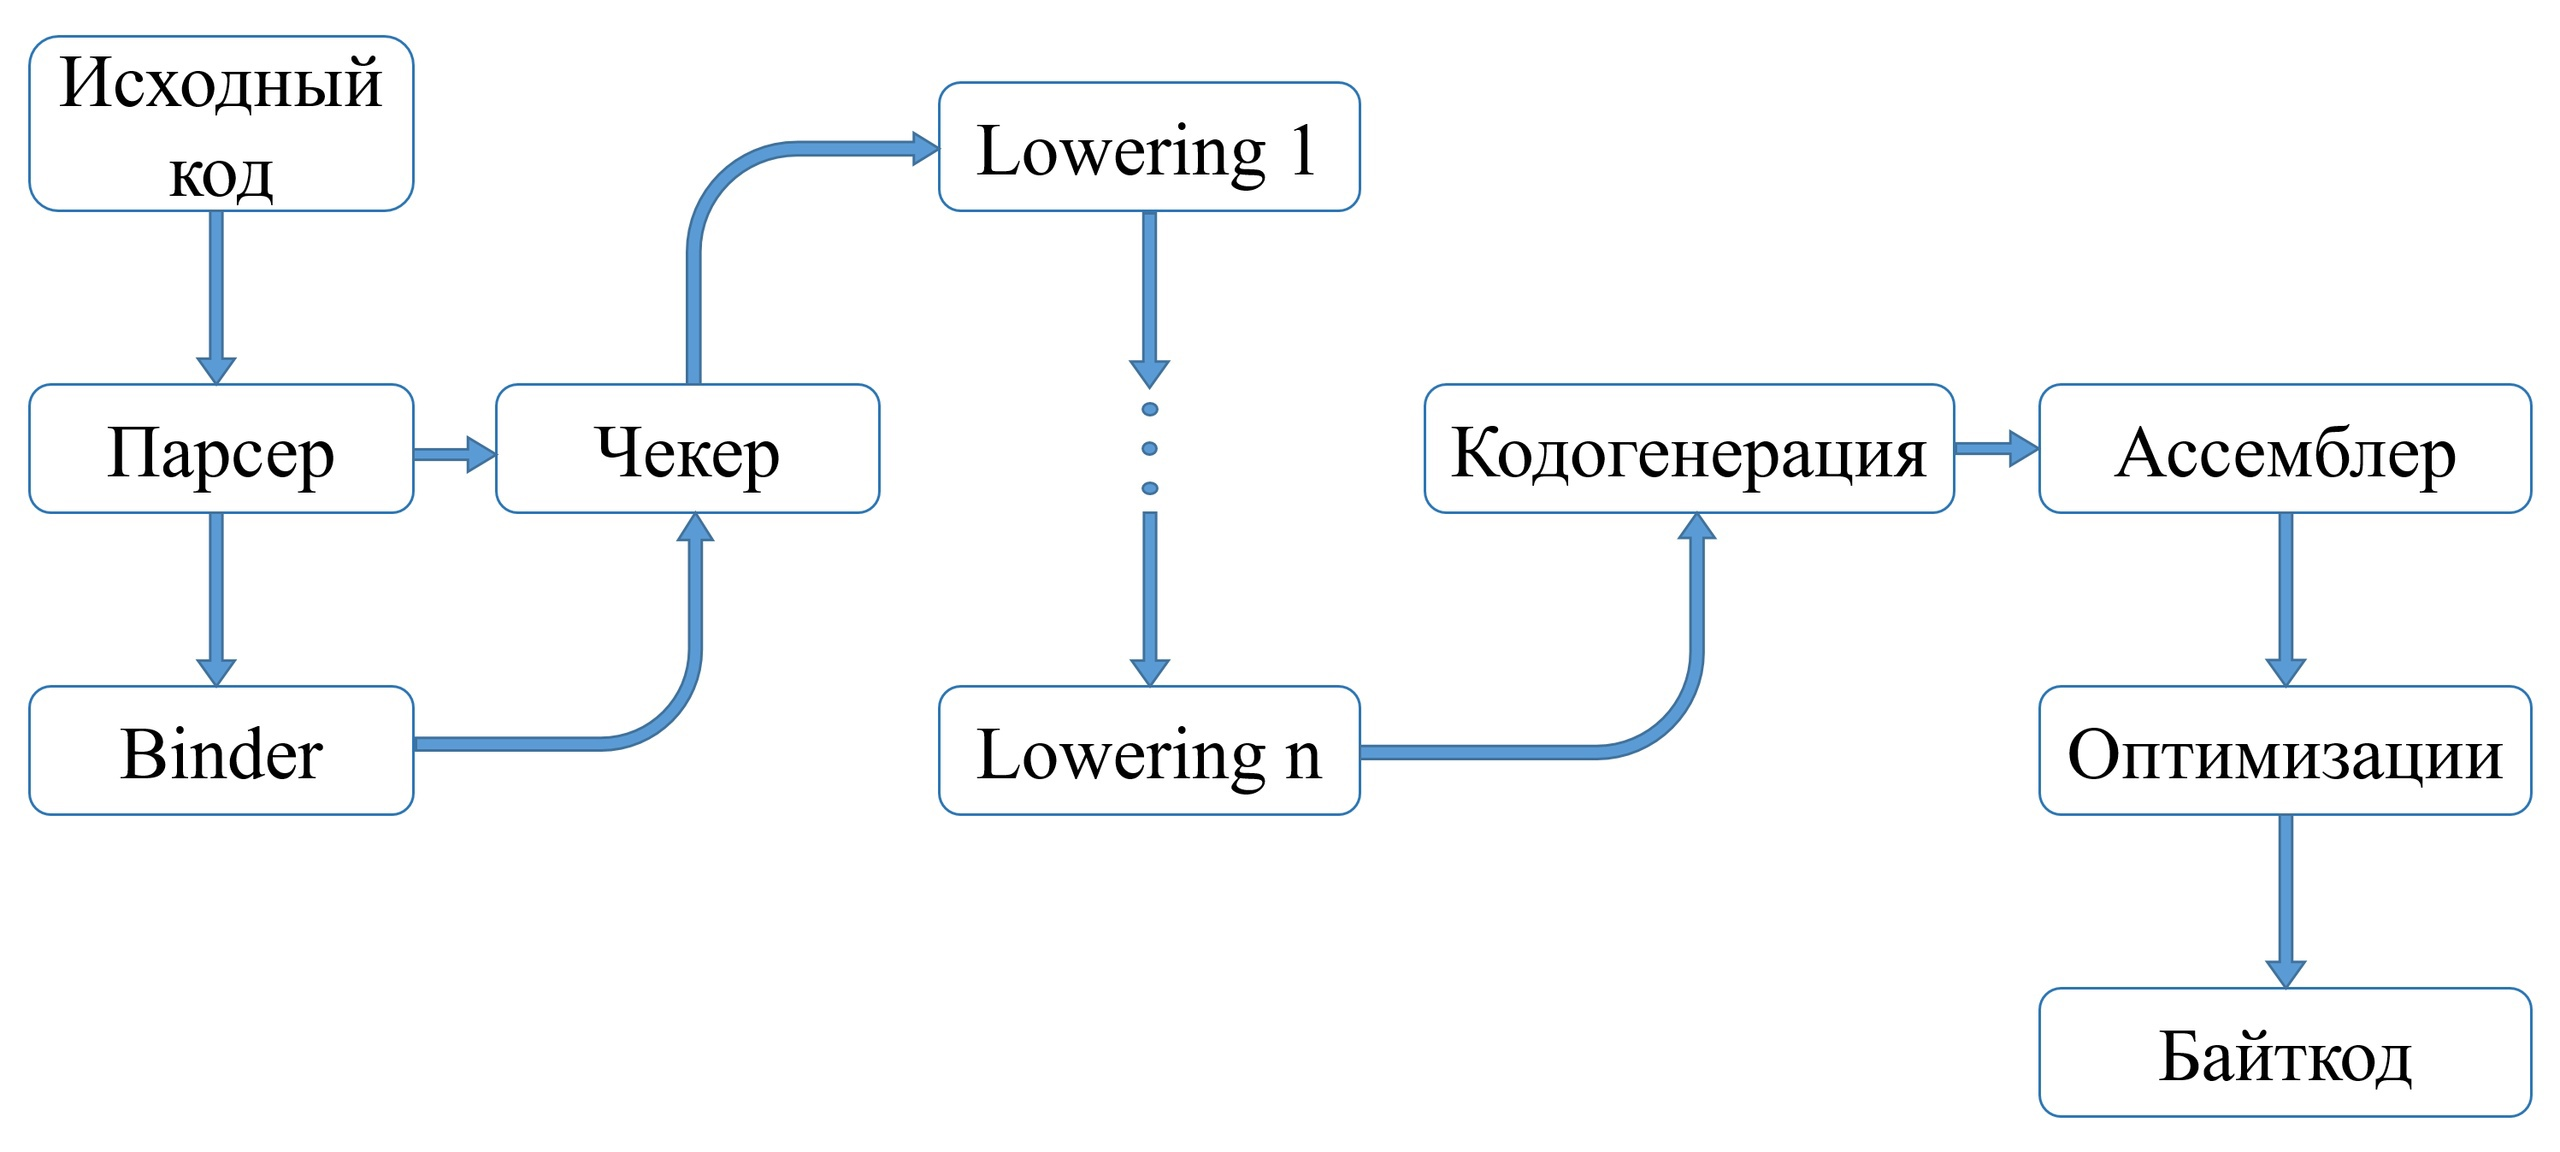
\includegraphics[scale=0.18]{Lowering1.jpg}
    \caption{Схема работы компилятора}\label{fig:figure}
\end{figure}

\subsection{Boxing и unboxing операции}

Boxing и unboxing - это важные концепции в языках программирования, особенно в тех, где есть поддержка
объектно-ориентированного программирования и системы типов.
Эти операции позволяют преобразовывать примитивные типы данных в объекты (boxing) и наоборот (unboxing), что
обеспечивает единообразное обращение к данным и их управление.

\subsubsection{Определения}

Boxing - это процесс преобразования примитивного типа данных в соответствующий ему объект.
Например, целочисленное значение типа int может быть упаковано в объект Integer в языке Java или в объект
System.Int32 в языке C\#.
Этот процесс автоматически осуществляется компилятором или средой выполнения.
Unboxing, наоборот, представляет собой процесс извлечения значения из упакованного объекта и его преобразования
обратно в примитивный тип данных.
Например, извлечение целочисленного значения из объекта Integer в Java или из объекта System.Int32 в C\#.

\subsubsection{Преимущества и Недостатки}

Одним из основных преимуществ использования boxing и unboxing является возможность работы с примитивными типами данных
в контексте объектно-ориентированного программирования.
Это позволяет использовать примитивные типы в качестве аргументов методов, сохранять их в коллекциях и передавать в
качестве параметров в методы, требующие объектов.
Однако, следует помнить, что процесс boxing и unboxing может быть затратным с точки зрения производительности, особенно
при выполнении операций в циклах или при работе с большими объемами данных.
Это связано с тем, что при упаковке и распаковке происходит создание дополнительных объектов и процесс их управления.

\subsubsection{Примеры в разных языках программирования}

Рассмотрим пример использования boxing и unboxing в языке программирования Java:
\begin{lstlisting}[language=Java,label={lst:lstlisting22}]
    int num = 10;
    Integer obj = num;

    Integer obj2 = new Integer(20);
    int num2 = obj2.intValue();
\end{lstlisting}
В первом случае на второй строке происходит автоматический boxing, а во втором на четвертой строке - явный unboxing.

В Kotlin также существует поддержка для boxing и unboxing, но благодаря удобным функциям и умному подходу к типизации,
эти операции редко требуются.
Однако, в некоторых случаях они могут быть полезны.
В Kotlin есть возможность использовать inline-функции и inline-классы, которые могут помочь избежать ненужных boxing и
unboxing.
Компилятор Kotlin может автоматически оптимизировать код, встроив вызовы функций и классов прямо в месте их использования.
Хорошая практика в языке способствует минимизации их использования в пользу примитивных типов и эффективных структур данных.

В TypeScript, поскольку это язык сильной типизации, прямого аналога операций boxing и unboxing, как в Java или C\#, нет.
Однако язык MyTS, используемый в нашей работе, статический и в нем присутствуют такие операции в отличие от TypeScript.
Поэтому при присвоении каких-то примитивных значений типу объединения придется использовать лишние вызовы для упаковки
или распаковки примитивов.
Мы постараемся в данной работе минимизировать такие дорогостоящие операции и оптимизировать байт-код под среду исполнения.

\subsection{Семантика и синтаксис объединений}

Для корректной поддержки семантики и синтаксиса TypeScript согласно поставленной задаче, необходимо изучить примеры
кода, где используются объединения, и спецификацию языка MyTS\@.
Рассмотрим описание объединений в исследуемом нами статически типизированном языке программирования и сравним их
функциональность с объединениями из TypeScript.

\subsubsection{Определение объединений}

Грамматика union типов задается тем же способом, что и в TypeScript, и может быть записана следующим образом:

\begin{lstlisting}
    unionType:
        type|literal ('|' type|literal)*
    ;
\end{lstlisting}
Здесь можно заметить, что компонентами объединения могут быть как обычные типы (пользовательские, встроенные,
примитивные, и т.д), так и литеральные, представляющие собой конкретные значения встроенных типов.
Все составляющие объединения должны быть перечислены через вертикальную черту.
Объединение является ссылочным типом, однако в данной работе мы сделаем определенное исключение для оптимизации кода.

Согласно спецификации, ошибка времени компиляции возникает, если тип в правой части объявления union типа приводит к
циклической ссылке.
Если в объединении используется примитивный тип, то выполняется автоматический boxing, чтобы сохранить
ссылочный характер типа.
Сокращенная форма объединения типов позволяет определить тип, который имеет только одно значение (литерал), например

\begin{lstlisting}
    type UT = 42
\end{lstlisting}

Рассмотрим различные примеры кода на TypeScript, которые будут валидны и в языке MyTS.

\subsubsection{Объединения с пользовательскими классами и доступ к полям}

Дадим определения некоторых пользовательских классов A, B и C:

\begin{lstlisting}
    class A {
        fieldA: number = 41
        field: number = 5
    }
    class B {
        fieldB: number = 42
        field: number = 6
    }
    class C {
        fieldC: number = 43
        field: number = 7
    }
\end{lstlisting}
То есть в каждом классе есть поле с именем field и одинаковым типом number, а также другое поле, уникальное для каждого
класса.
Тогда мы имеем право создать следующие псевдонимы (type alias) на объединения пользовательских классов с примитивным типом
number и без него:

\begin{lstlisting}
    type UT1 = A|B|C|number
    type UT2 = A|B|C
\end{lstlisting}
где UT1 может быть экземпляром класса A, B, C или числом, а UT2 может быть экземпляром класса A, B или C\@.
Далее рассмотрим фрагменты кода, которые используют определенные нами типы объединения.

\begin{lstlisting}
    let u1: UT1 = new A();
\end{lstlisting}
Здесь переменной u1 присваивается тип UT1, и ей присваивается экземпляр класса A\@.
На этом этапе u1 конкретно является типом A\@.
Рассмотрим доступ к свойству field:
\begin{lstlisting}[escapechar=!]
    u1.!\colorbox{lightcoral}{field}!
\end{lstlisting}
TypeScript здесь обязан выдать ошибку, потому что u1 может потенциально быть числом, а число не имеет свойства field.
Чтобы безопасно получить доступ к свойству field, нужно сузить тип переменной:

\begin{lstlisting}
    if (u1 instanceof A) {
        u1.fieldA
        (u1 as A).fieldA
    }
    u1 = 45
\end{lstlisting}
Условие \hl{if (u1 instanceof A)} сужает тип u1 до A внутри блока.
Внутри этого блока \hl{u1.fieldA} и \hl{(u1 as A).fieldA} оба безопасно получают доступ к fieldA\@.
После чего значение 45 типа number присваивается переменной u1, что допустимо, поскольку UT1 включает тип number.
Рассмотрим пример использования u2:

\begin{lstlisting}
    let u2: UT2 = new C()
    u2.field
\end{lstlisting}
Здесь u2 имеет тип UT2, и ей присваивается экземпляр класса C.
Поскольку u2 может быть только A, B или C, доступ к u2.field безопасен, потому что все эти классы имеют свойство field
с одним и тем же типом поля number.

Фрагменты кода выше показывают, как объединённые типы TypeScript, сужение типов с помощью instanceof и приведения типов
(as) работают вместе для обеспечения безопасности типов и гибкости кода.

\subsubsection{Объединения с литералами}

Дадим определения следующих псевдонимов для объединений литеральных типов:

\begin{lstlisting}
    type UT3 = 5
    type UT4 = 5 | 7 | 9
\end{lstlisting}
где UT3 — это литеральный тип, который может принимать только значение 5, а UT4 — это объединение, которое может
принимать только конкретные значения 5, 7 или 9.
Рассмотрим использование типа UT3:

\begin{lstlisting}[escapechar=!]
    let u3: UT3 = 5
    !\colorbox{lightcoral}{u3}! = 4
\end{lstlisting}
Здесь переменной u3, имеющей тип UT3, сначала присваивается значение 5.
Это допустимо, поскольку UT3 может быть только литералом 5.
Однако на следующей строчке TypeScript выдаёт ошибку, потому что u3 может принимать только значение 5, и попытка
присвоить ей 4 недопустима.
Далее рассмотрим использование типа UT4:
\begin{lstlisting}
    let u4: UT4 = 5
    if (u4 == 5) {
        u4 = 7;
    } else if (u4 == 7) {
        u4 = 9;
    }
\end{lstlisting}
Здесь переменной u4 присваивается тип UT4, и ей присваивается значение 5.
Это допустимо, поскольку UT4 может иметь значения литералов 5, 7 или 9.
Далее в условном ветвлении идет проверка значения u4 на равенство какому-либо литералу, после чего оно изменяется в
зависимости от результата проверки.
Если u4 равно 5, то ему присваивается значение 7.
Если u4 равно 7, то ему присваивается значение 9.
В любом случае эти присваивания допустимы, так как 7 и 9 входят в допустимый диапазон значений типа UT4.
Однако, если мы попытаемся сравнить значение u4 с литералом, которого нет в объединении, то согласно спецификации
должна произойти ошибка времени компиляции для такого кода:
\begin{lstlisting}
    u4 == 99
\end{lstlisting}

Эти примеры демонстрируют, как TypeScript использует литеральные и объединённые типы для обеспечения строгой типизации
и контроля значений переменных.

\subsubsection{Нормализация объединений}

Нормализация объединённых типов позволяет минимизировать количество типов и литералов в объединённом типе, сохраняя
при этом безопасность типа.
Некоторые типы или литералы могут быть также заменены на более общие типы.
Формально, объединённый тип $A_1$ | \ldots | $A_n$, где N > 1, может быть сокращён до типа $B_1$ | \ldots | $B_k$, где k <= n,
или даже до не объединённого типа или значения T\@.
В последнем случае T может быть примитивным типом или литералом, изменяющим ссылочную природу типа объединения.

Процесс нормализации предполагает выполнение следующих шагов один за другим:

\begin{itemize}[left=2em]
    \item Линеаризация: Если объединение состоит из двух или более вложенных объединений, они сливаются в одно объединение.
    Например,

    \hl{($A_1$ | $A_2$) | ($A_3$ | $A_4$)} превращается в \hl{$A_1$ | $A_2$ | $A_3$ | $A_4$}.
    \item Удаление идентичных типов: Если в объединении есть несколько одинаковых типов, то они сокращаются до одного.
    Например,

    \hl{string | string} превращается в \hl{string}.

    То же после boxing: Если один тип в объединении может быть преобразован в другой через boxing, то они заменяются на
    более общий тип.
    Например, \hl{number | Number} становится \hl{Number}.
    \item Удаление идентичных значений: Если в объединении есть несколько одинаковых литералов, они сокращаются до одного.

    Например, \hl{5 | 5 | 5} превращается в \hl{5}.
    \item Доминирование Object: Если в объединении есть тип Object, то все остальные не-nullish типы удаляются.

    Например, \hl{777 | Object} становится \hl{Object}.
    \item Если среди объединённых типов присутствует тип never, то он удаляется (\hl{number | never} => \hl{number}).
    \item Если в объединении есть непустая группа числовых типов, то в объединении остаётся только самый крупный числовой тип,
    а остальные удаляются.
    Любой числовой литерал, который подходит под самый крупный числовой тип в объединении, удаляется.
    Другими словами, если в объединении есть числовые типы, то остаётся наибольший из них.
    Например, \hl{int | short | float | 2} становится \hl{float}.
    \item Удаление литералов, принадлежащих типам: Если литерал принадлежит типу, который является частью объединения,
    то он удаляется.
    Например, \hl{5 | number} превращается в \hl{number}.
    \item Удаление литералов, принадлежащих unboxed типам чисел: Если числовой литерал принадлежит unboxed типу одного
    из объединённых числовых типов, он удаляется.
    Например, \hl{Int | 3.14 | Float} превращается в \hl{Int | Float}.
    \item Доминирование базового типа в иерархии классов: Если в объединении есть класс и его производный класс,
    то побеждает базовый класс.
    Например:
        \begin{lstlisting}
            class Base {}
            class Derived1 extends Base {}
            class Derived2 extends Base {}
            Base | Derived1 => Base
            Derived1 | Derived2 => Derived1 | Derived2
        \end{lstlisting}
    \item Этот шаг выполняется рекурсивно до тех пор, пока не останется взаимно совместимых типов или пока объединённый
    тип не сократится до одного типа:
    \begin{itemize}[left=2em]
        \item Если объединённый тип включает два типа $A_i$ и $A_j$ (i != j), и $A_i$ совместим с $A_j$, то в объединённом типе
    остаётся только $A_j$, а $A_i$ удаляется.
        \item Если $A_j$ совместим с $A_i$, то в объединённом типе остаётся $A_i$, а $A_j$ удаляется.
    \end{itemize}
\end{itemize}

Результатом процесса нормализации является либо нормализованный union тип, либо один единственный тип, не являющийся
объединением, причем он может быть и не ссылочным типом.

\subsection{Инструкция для доступа к полю объединения}

Для более эффективной генерации байт-кода, в архитектуре системы команд (ISA), данной нам среде исполнения, предусмотрены
специальные инструкции:

\begin{itemize}[left=2em]
    \item LON\_INST (Load Object field by Name Instruction) - загрузка в аккумулятор поля объекта по имени
    \item SON\_INST (Store something into Object field by Name Instruction) - загрузка значения
    из аккумулятора в поле объекта
\end{itemize}

Для того, чтобы инструкция в среде исполнения отработала корректно, необходимо сгенерировать специальный класс в
байт-коде, который называется \hl{union\_member\_access}.
В этом классе должно быть объявлено поле с тем именем и типом, которое существует для всех компонент объединения.
Позже среда исполнения сможет получить доступ к полю объединения на основе этих данных, несмотря на то
какой конкретно тип объекта хранится в объединении, причем без приведения к более узкому типу.

\newpage
